\maketitle

\cleardoublepage
\phantomsection
\addcontentsline{toc}{chapter}{Indice}
\tableofcontents

\listoffigures

\chapter{Introduzione}
\textsl{\textbf{Climate Monitoring}} è un'applicazione sviluppata nell’ambito del progetto di Laboratorio InterdisciplinareB (A.A. 2023/24) per il corso di laurea in Informatica dell’\textsl{Universit\`a degli Studi dell’Insubria} di Varese.

Il progetto è sviluppato in \textsl{Java 17} sui sistemi operativi \textsl{Arch Linux} e \textsl{Windows 11}.
L'applicazione è stata testata sugli stessi sistemi.

Questo manuale descrive la struttura del progetto e delle risorse che utilizza. Per avere informazioni più dettagliate consultare la JavaDoc del codice sorgente.

\section{Librerie in Comune al Client e al Server Utilizzate}

Per lo sviluppo di questo progetto sono state utilizzate alcune librerie di terze parti.

Per le librerie specifiche al client (Capitolo \ref{ch:client}) e al server (Capitolo \ref{ch:server}) riferirsi ai capitoli appropriati.

\subsection{\textsl{Lombok}}

\href{https://projectlombok.org/}{Sito progetto}

Il progetto Lombok mira a ridurre la quantità di codice scritto tramite annotazioni che si attivano a tempo di compilazione.

\subsection{\textsl{Apache Log4j}}

\href{https://logging.apache.org/log4j/2.x/}{Sito progetto}

Abbiamo usato \textsl{Log4j} per via della sua popolarità e comprovata robustezza.

\chapter{Database (dbCM)}
Di seguito si mostra lo schema Entità-Relazione del database di supporto all’esecuzione dei servizi della piattaforma Climate Monitoring.

\begin{figure}[h]
	\centering
	\caption{Schema ER del database}
	\label{fig:erdb}
	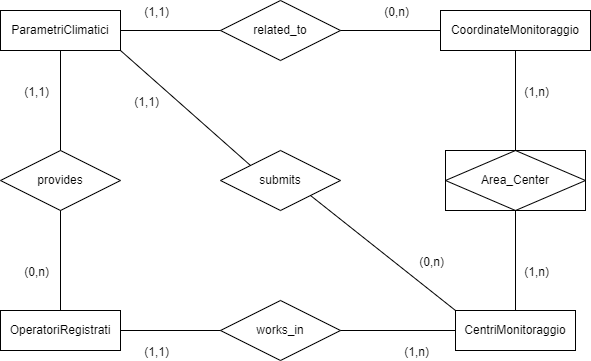
\includegraphics[width=0.8\linewidth]{../../fig/img/tecnico/ERdb.drawio}
\end{figure}


In questo schema vegono illustrate le entità richieste dalle specifiche e le relative associazioni.

Nel dettaglio:
\begin{itemize}
	\item \textbf{\textit{CentriRegistrati}}, contenente tutte le informazioni relative ai centri di monitoraggio registrati nel sistema, creati dai vari operatori;
	\item \textbf{\textit{CoordinateMonitoraggio}}, contenente i dati riguardanti le aree geografiche presenti nel documento "CoordinateMonitoraggio.xlsx" fornito nelle specifiche di progetto;
	\item \textbf{\textit{OperatoriRegistrati}}, racchiude i dettagli relativi gli operatori che hanno effettuato la registrazione al sistema;
	\item \textbf{\textit{ParametriClimatici}}, modella dei record per contenere tutte le informazioni che interessano le misurazioni effettuate in determinate aree d'interesse dagli operatori registrati, per conto dei relativi centri di monitoraggio.
\end{itemize}
\pagebreak
Le associazioni costruite sulle entità appena elencate sono le seguenti:
\begin{itemize}
	\item \textbf{\textit{"provides"}}, tra \textit{OperatoriRegistati} e \textit{ParametriClimatici}, con cardinalità \textbf{\textit{(0,n)-(1,1)}}
	      
	      Ogni operatore registrato può difatti fornire più misurazioni climatiche, mentre una misurazione può essere stata fornita da uno e un solo operatore registrato.
	\item \textbf{\textit{"related\_to"}}, tra \textit{ParametriClimatici} e \textit{CoordinateMonitoraggio}, con cardinalità \textbf{\textit{(1,1)-(0,n)}}
	      
	      Ogni misurazione climatica deve difatti essere relativa a una e una sola area geografica, mentre un'area geografica può avere associate molteplici misurazioni, come non averne.
	\item \textbf{\textit{"submits"}}, tra \textit{CentriMonitoraggio} e \textit{ParametriClimatici}, con cardinalità \textbf{\textit{(0,n)-(1,1)}}
	      
	      Ogni centro di monitoraggio può presentare più misurazioni relative alle proprie aree d'interesse, mentre una misrurazione deve essere stata resa disponibile da uno e un solo centro di monitoraggio.
	\item \textbf{\textit{"works\_in"}}, tra \textit{OperatoriRegistrati} e \textit{CentriMonitoraggio}, con cardinalità \textbf{\textit{(1,1)-(1,n)}}
	      
	      Ogni operatore deve associarsi a un centro di monitoraggio in seguito alla registrazione, se quello a cui vuole associarsi non è presente nel sistema, ne crea uno nuovo. In ogni centro di monitoraggio lavora almeno un operatore (il suo creatore), ed eventualmente altri associati.
	\item \textbf{\textit{"Area\_Center"}}, tra \textit{CoordinateMonitoraggio} e \textit{CentriMonitoraggio}, con cardinalità \textbf{\textit{(1,n)-(1,n)}}
	      
	      Ogni area geografica può essere considerata d'interesse da più centri di monitoraggio, i quali a loro volta possono monitorare molteplici aree d'interesse.
	      Sulla base di questa associazione, in seguito alla ristrutturazione dello schema ER è stata costruita un'ulteriore relazione omonima, trattandosi di un'associazione di tipo "molti a molti".
\end{itemize}
Escludendo quest'ultima, le prime 4 associazioni mostrate (trattandosi di assocazioni di tipo "uno a molti"/"molti a uno") sono state invece riportate nello schema relazionale come vincoli di chiave esterna.
\pagebreak

Il seguente schema relazionale mostra nel dettaglio gli attributi (con i vari tipi associati) di ogni relazione e i relativi vincoli di chiave primaria ed esterna.

\begin{figure}[h]
	\centering
	\caption{Schema dettagliato del database}
	\label{fig:quickdbd-clima}
	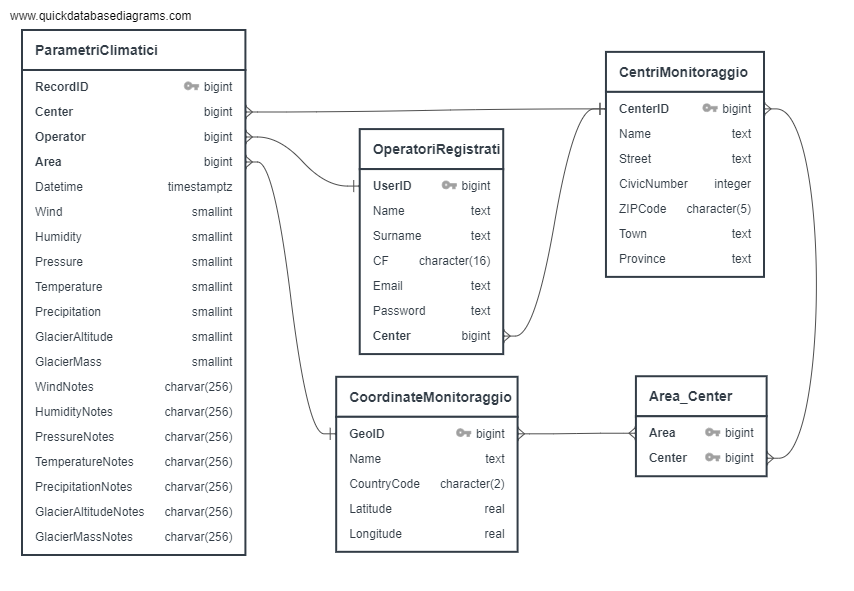
\includegraphics[width=0.8\linewidth]{../../fig/img/tecnico/QuickDBD-clima}
\end{figure}

Gli attributi di ogni relazione sono stati inseriti sulla base delle indicazioni fornite nel documento delle specifiche di progetto. Al riguardo, sono degne di nota le seguenti scelte progettuali:
\begin{itemize}
	\item in \textit{\textbf{ParametriClimatici}}, è stato aggiunto l'attributo \textit{"RecordID"}, utilizzato come chiave primaria della relazione, in modo da usufruire di un identificatore univoco per ogni record che riguarda le misurazioni climatiche; inoltre gli attributi riguardanti le note dei parametri di rilevazione non sono stati dichiarati \textit{"NULLABLE"}, in quanto l'eventuale mancanza di tali dati (opzionali) è stata gestita a livello applicativo tramite l'uso di stringhe vuote;
	\item in \textit{\textbf{CoordinateMonitoraggio}}, gli attributi \textit{"Latitude"} e \textit{"Longitude"} sono stati separati, nonostante nel documento \textit{"CoordinateMonitoraggio.xlsx"} (fornito nelle specifiche di progetto, sulla base del quale è stata costruita questa relazione) siano parte dello stesso campo \textit{"Coordinates"}, in modo da facilitarne la manipolazione a livello applicativo.
\end{itemize}

\chapter{Modulo \texttt{org.a3b.clientCM}}
Il modulo clientCM gestisce il lato client dell'applicazione.
\label{ch:client}
\section{Librerie Utilizzate dal Client}

\chapter{Modulo \texttt{org.a3b.serverCM}}
Il modulo clientCM gestisce il lato server dell'applicazione.
\label{ch:server}
\begin{figure}[h]
	\centering
	\caption{Struttura del modulo serverCM}
	\label{fig:severcm}
	\includegraphics[width=0.9\linewidth]{../../fig/img/tecnico/ServerCM.drawio}
\end{figure}
\pagebreak

Come si può notare dal diagramma, comprende:
\begin{itemize}
	\item classe \textbf{\texttt{ServerCM}}
		Si occupa della connessione RMI per rendere il sistema distribuito e della connessione con il database.
	\item classe \textbf{\texttt{DataFactory}}
		Contiene metodi che permettono di creare le varie istanze d'interesse a partire da record estratti dal database. 
	\item classe \textbf{\texttt{ServerImpl}}
		Implementazione vera e propria del server, estende \texttt{UnicastRemoteObject} (per essere inserita nel registry di RMI) e implementa l'interfaccia \texttt{ServicesCM}, che contenente tutte le funzioni richieste (Capitolo \ref{ch:commons}).
\end{itemize}

\section{Librerie Utilizzate dal Server}
\begin{itemize}
	\item \texttt{java.rmi}, per rendere il sistema distribuito:
		\begin{itemize}
			\item \texttt{RemoteException}
			\item \texttt{server.UnicastRemoteObject}
			\item \texttt{registry.LocateRegistry}
			\item \texttt{registry.Registry}
		\end{itemize}
	\item \texttt{java.sql}, per supportare le operazioni che coinvolgono il database:
		\begin{itemize}
			\item \texttt{ResultSet}
			\item \texttt{SQLException};
			\item \texttt{Timestamp}
			\item \texttt{Connection}
			\item \texttt{DriverManager}
		\end{itemize}
	\item \texttt{java.util}:
	\begin{itemize}
		\item \texttt{Objects}
		\item \texttt{Properties}
	\end{itemize}
	
\end{itemize}

\chapter{Modulo \texttt{org.a3b.commons}}
\label{ch:commons}
Commons contiene e gestisce l'insieme di risorse utilizzate sia dal modulo clientCM che da serverCM.
\begin{figure}[h]
	\centering
	\caption{Struttura del modulo commons}
	\label{fig:commonscm}
	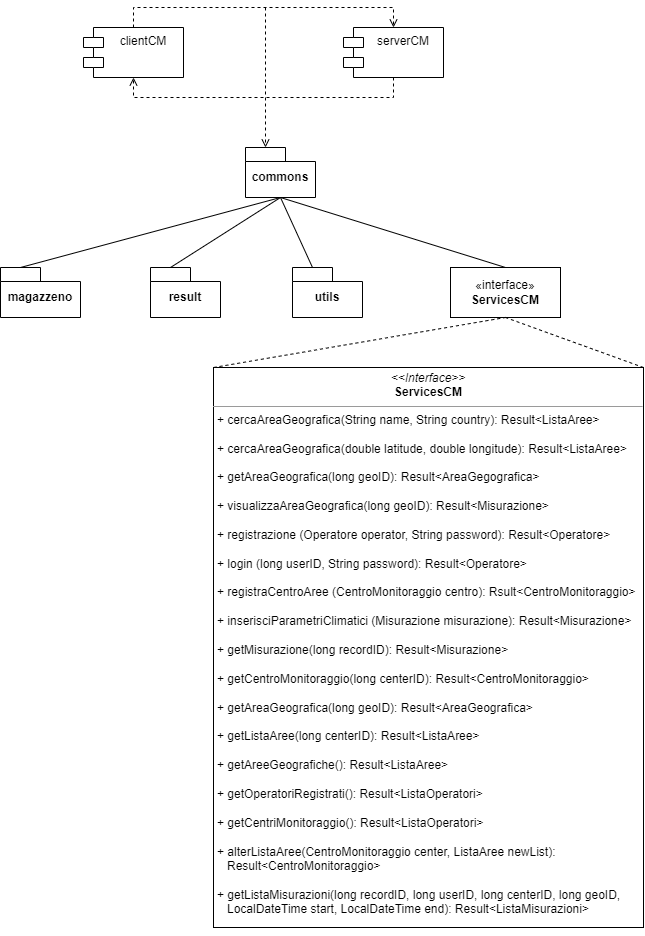
\includegraphics[width=0.85\linewidth]{../../fig/img/tecnico/CM.drawio}
\end{figure}


Come si può notare dal diagramma, comprende:
\begin{itemize}
	\item package \textbf{\texttt{magazzeno}}
		
		Contiene le classi che modellano le istanze gestite dal sistema, in particolare:
		\begin{itemize}
			\item \texttt{AreaGeografica}, rappresenta un'area di interesse per la rilevazione di parametri climatici;
			\item \texttt{CentroMonitoraggio}, rappresenta un centro di monitoraggio;
			\item \texttt{ListaAree}, rappresenta una lista di aree geografiche associate a un determinato centro di monitoraggio;
			\item \texttt{Misurazione}, rappresenta il risultato di una rilevazione climatica;
			\item \texttt{Operatore}, rappresenta un operatore dei centri di monitoraggio.
		\end{itemize}
	\item package \textbf{\texttt{result}}
		
		Modella un "contenitore" utilizzato per una gestione migliore dei possibili errori generati all'interno dell'applicazione.
		Per ulteriori informazioni consultare i relativi codice sorgente e JavaDoc.
	\item package \textbf{\texttt{utils}}
		
		Contiene elementi che facilitano la lettura e l'organizzazione del codice, in particolare:
		\begin{itemize}
			\item interfaccia \texttt{CercaAree}, per la ricerca di aree geografiche;
			\item interfaccia \texttt{MediaAree}, per il calcolo della media dei valori assegnati ai parametri climatici;
			\item enumerativo \texttt{TipoDatoGeogafico}, modella i vari parametri di ogni rilevazione climatica.
		\end{itemize}
	\item interfaccia \textbf{\texttt{ServicesCM}}
	
		Racchiude tutte i metodi forniti dal server e utilizzate dal client. In particolare sono presenti tutte le funzioni richieste dalle specifiche di progetto.
\end{itemize}

\nocite{IuriTex}
\bibliographystyle{alpha}
\bibliography{bib/biblio}
